\documentclass{book}
\usepackage[T1]{fontenc}
\usepackage[utf8]{inputenc}
\usepackage[LGR,T1]{fontenc} % notice LGRx instead of LGR
\usepackage{lmodern}
\usepackage[final]{pdfpages} 
\usepackage[top=2cm, bottom=3cm, outer=3cm, inner=4cm, headsep=14pt]{geometry}
\usepackage{textgreek}
\usepackage{csquotes}
\usepackage[french]{babel}
\usepackage{fancyhdr}
\usepackage{xsim}
\usepackage{tasks}
\usepackage[absolute]{textpos}
\usepackage{ascii}
\usepackage{eurosym}
\usepackage{amsthm}
\usepackage{url}
\usepackage{circuitikz}
\usepackage{float}
\usepackage{pdfpages}
\usepackage{multirow}
\usepackage{xcolor,colortbl}
\usepackage{amsmath}


\theoremstyle{definition}
\newtheorem{exmp}{Example}[section]

\bibliographystyle{abbrv}
\pagestyle{fancy}
\fancyhf{}
\renewcommand{\footrulewidth}{1pt}
\renewcommand{\thesection}{\arabic{section}}

\theoremstyle{definition}
\newtheorem{definition}{Definition}[section]

\lhead{Architecture des ordinateurs}
\rhead{Systèmes logiques}
\rfoot{Page \thepage}

\begin{document}
\chapter{Systèmes logiques}
Dans ce chapitre, nous allons, à partir de tout ce qui a été vu précédemment, réaliser des circuits logiques qui proposent des fonctions logiques parmi les plus communément utilisées. Ces exemples sont issus de différents domaines : électronique industrielle, fonction de calcul, etc.

\section{Additionneur}
Comme pour les additions en décimal, nous allons décomposer l'addition par colonnes.
\\

\begin{tabular}{ c|c }
 19 & 0001 0011 \\
 50 & 0011 0010 \\
 \hline
 69 & 0100 0101 \\
\end{tabular}
\\

\subsection{Demi-additionneur}
Pour la première colonne, c'est-à-dire l'addition sur le premier bit avec retenue de $A_0$ et $B_0$, nous avons la table de vérité suivante\footnote{Nous avons en fait combiné deux tables de vérités, pour deux sorties, par souci de simplicité.} avec la sortie S pour la somme et la sortie C pour la retenue (en anglais \textit{carry}) :
\\

  \begin{tabular}{|c|c||c|c|}
    \hline
         \multicolumn{2}{|c||}{Entrées}& \multicolumn{2}{c|}{Sorties}\\
        
        $A_0$ & $B_0$ & $S=A\oplus B$ & $C=A\cdot B$ \\
    \hline 
        0 & 0 & 0 & 0\\
        0 & 1 & 1 & 0\\
        1 & 0 & 1 & 0\\
        1 & 1 & 0 & 1\\
    \hline
  \end{tabular}
\\

La réalisation du circuit logique est immédiate comme on peut le voir sur la figure \ref{fig:demiadd}.


\begin{figure}
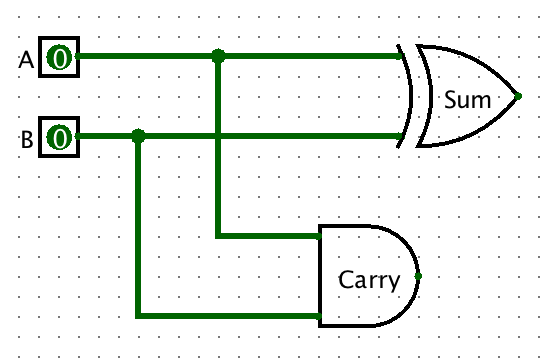
\includegraphics[width=0.5\textwidth]{media/SysLogiques/DemiAdd.png}
    \centering
    \caption{Demi-additionneur}
    \label{fig:demiadd}
\end{figure}


\subsection{Additionneur complet}
Pour le bit de poids $n$, nous devons maintenant prendre en compte la retenue du bit de poids $n-1$ que nous appellerons ici $C_{in}$ et nous appellerons $C_{out}$ la retenue en sortie. La table de vérité devient ainsi, avec trois entrées :
\\

  \begin{tabular}{|c|c|c||c|c|}
    \hline
         \multicolumn{3}{|c||}{Entrées}& \multicolumn{2}{c|}{Sorties}\\
        
         $A_n$ & $B_n$ & $C_{in}$ & $S_n$ & $C_{out}$ \\
    \hline 
        0 & 0 & 0 & 0 & 0\\
        0 & 0 & 1 & 1 & 0\\
        0 & 1 & 0 & 1 & 0\\
        0 & 1 & 1 & 0 & 1\\
        1 & 0 & 0 & 1 & 0\\
        1 & 0 & 1 & 0 & 1\\
        1 & 1 & 0 & 0 & 1\\
        1 & 1 & 1 & 1 & 1\\
    \hline
  \end{tabular}

Le circuit pour l'additionneur complet est donc composé de deux demi-additionneurs, auquel on adjoint la logique nécessaire au calcul de la retenue. On peut voir cet additionneur à la figure \ref{fig:add}.

\begin{figure}
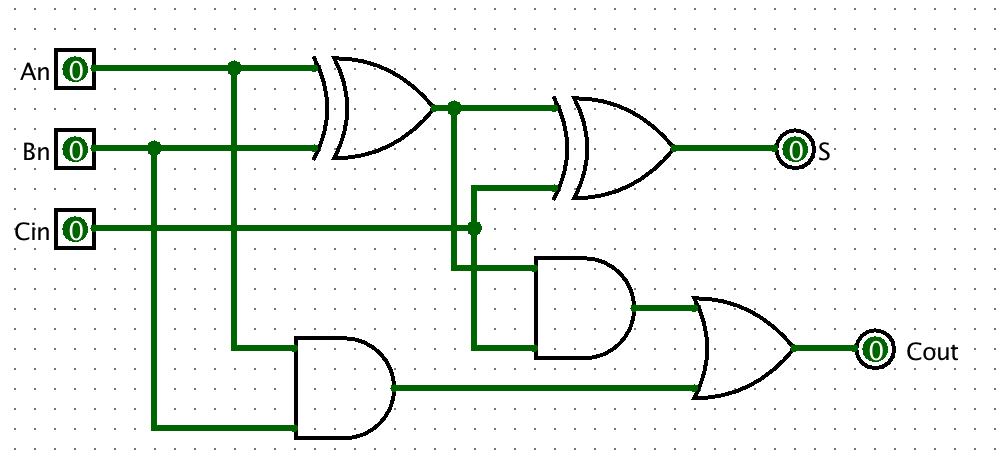
\includegraphics[width=0.5\textwidth]{media/SysLogiques/Add.png}
    \centering
    \caption{Additionneur complet}
    \label{fig:add}
\end{figure}

On peut maintenant "chaîner" des "boites" d'additionneurs pour obtenir un additionneur sur le nombre de bits souhaité. On voit par exemple sur la figure \ref{fig:add4bit} un additionneur 4bits.

\begin{figure}
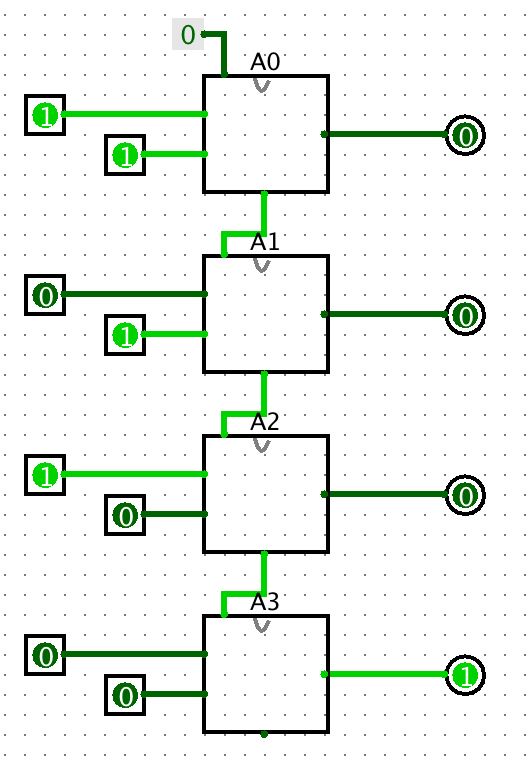
\includegraphics[width=0.5\textwidth]{media/SysLogiques/add4bit.png}
    \centering
    \caption{Additionneur 4 bits}
    \label{fig:add4bit}
\end{figure}

L'additionneur étant au coeur des unités arithmétiques et logiques des micro-processeur, il a fait l'objet d'études et d'optimisations particulières. Le lecteur qui souhaite en savoir plus se référera (pour commencer) à la page wikipedia sur l'additionneur.
\section{Inverseur}
Nous parlons ici de l'inversion d'un nombre en complément à deux pour trouver sa représentation négative (et non d'une inversion bit à bit pour laquelle la solution est immédiate).
Le complément à deux s'obtient donc en inversant tous les bits et en ajoutant 1 pour obtenir un nombre négatif.
En utilisant l'additionneur vu précédement avec des entrées constantes, on obtient ainsi sur les figures \ref{fig:inv0}, \ref{fig:inv1} et \ref{fig:inv6} la représentation en complément à deux de respectivement 0, 1 et 6.

\begin{figure}
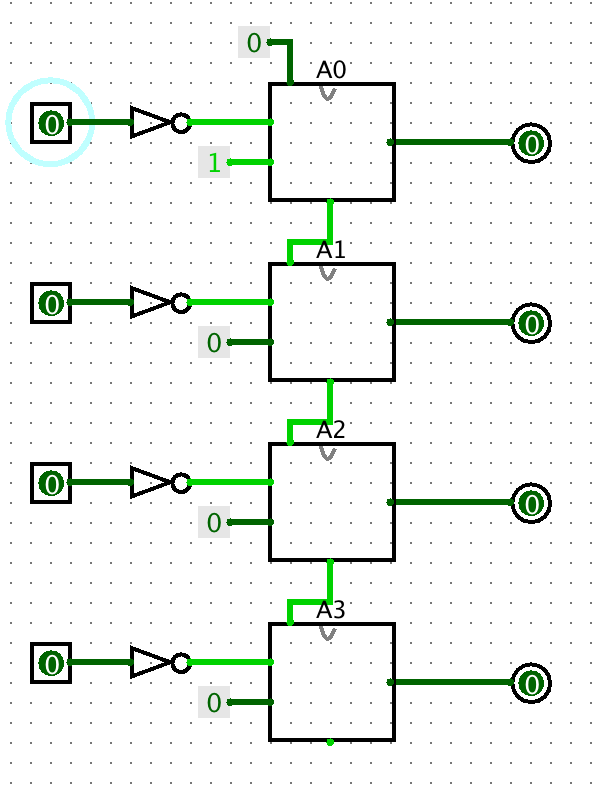
\includegraphics[width=0.5\textwidth]{media/SysLogiques/inv0.png}
    \centering
    \caption{-0}
    \label{fig:inv0}
\end{figure}

\begin{figure}
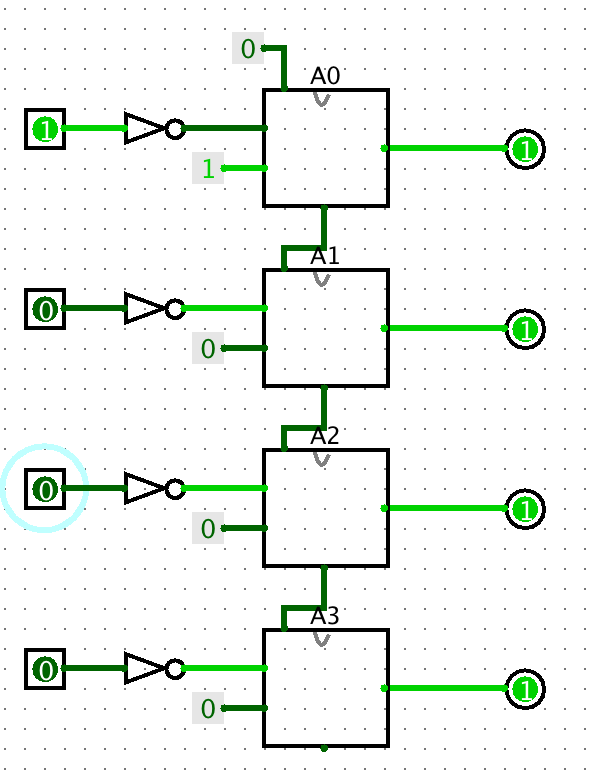
\includegraphics[width=0.5\textwidth]{media/SysLogiques/inv1.png}
    \centering
    \caption{-1}
    \label{fig:inv1}
\end{figure}

\begin{figure}
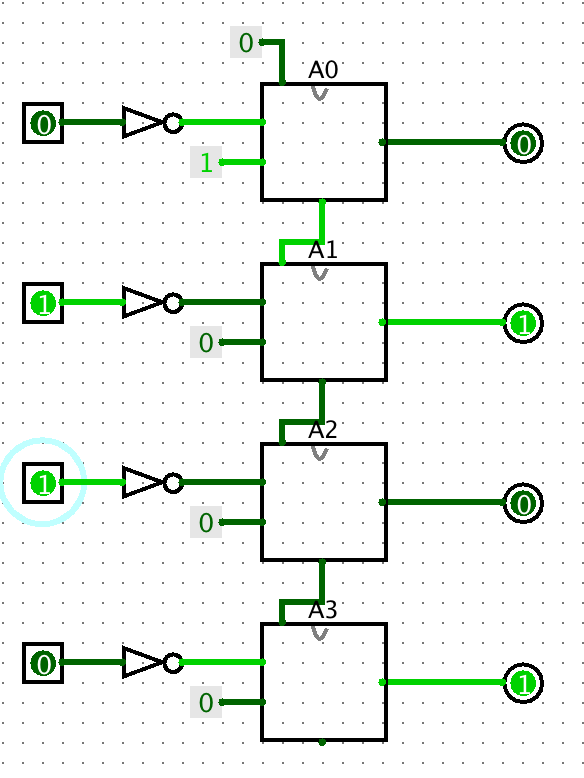
\includegraphics[width=0.5\textwidth]{media/SysLogiques/inv6.png}
    \centering
    \caption{-6}
    \label{fig:inv6}
\end{figure}

\section{Affichage sept segments}
On appelle affichage sept segments un affichage numérique composé de sept diodes qui peuvent être commandées individuellement. Ces circuits coûtent en général quelques euros. Une huitième diode est parfois ajoutée pour représenter le point décimal, mais nous n'en tiendrons pas compte dans la suite de la discussion. On voit sur la figure \ref{fig:7seg} comment sont désignés (habituellement) les huit segments de a à g.

\begin{figure}
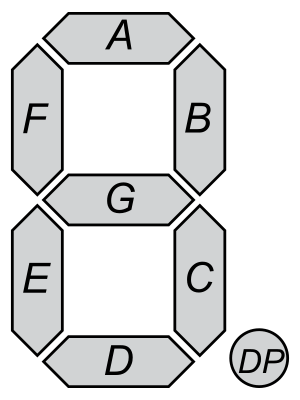
\includegraphics[width=0.5\textwidth]{media/SysLogiques/7seg.png}
    \centering
    \caption{Affichage sept segments}
    \label{fig:7seg}
\end{figure}

Un demi-octet représentant des nombres décimaux de 0 à 15, on utilise souvent de tels dispositifs pour afficher les nombres en hexadécimal. Il faut donc établir un circuit logique pour représenter un demi-octet en allumant les diodes correspondantes. Pour cela, nous établissons la table de vérité suivante :
\\

 \begin{tabular}{|c||c|c|c|c||c|c|c|c|c|c|c|c|}
    \hline
         Nombre &
         \multicolumn{4}{c||}{Demi-octet}& \multicolumn{7}{c|}{Sorties}\\
        
         $N$ & $N_3$ & $N_2$ & $N_1$ & $N_0$ & a & b & c & d & e & f & g\\
    \hline 
        0 & 0 & 0 & 0 & 0 & 1 & 1 & 1 & 1 & 1 & 1 & 0 \\
        1 & 0 & 0 & 0 & 1 & 0 & 1 & 1 & 0 & 0 & 0 & 0 \\
        2 & 0 & 0 & 1 & 0 & 1 & 1 & 0 & 1 & 1 & 0 & 1 \\
        3 & 0 & 0 & 1 & 1 & 1 & 1 & 1 & 1 & 0 & 0 & 1 \\
    \hline
        4 & 0 & 1 & 0 & 0 & 0 & 1 & 1 & 0 & 0 & 1 & 1 \\
        5 & 0 & 1 & 0 & 1 & 1 & 0 & 1 & 1 & 0 & 1 & 1 \\
        6 & 0 & 1 & 1 & 0 & 0 & 0 & 1 & 1 & 1 & 1 & 1 \\
        7 & 0 & 1 & 1 & 1 & 1 & 1 & 1 & 0 & 0 & 0 & 0 \\
    \hline
        8 & 1 & 0 & 0 & 0 & 1 & 1 & 1 & 1 & 1 & 1 & 1 \\
        9 & 1 & 0 & 0 & 1 & 1 & 1 & 1 & 0 & 0 & 1 & 1 \\
        A & 1 & 0 & 1 & 0 & 1 & 1 & 1 & 0 & 1 & 1 & 1 \\
        b & 1 & 0 & 1 & 1 & 0 & 0 & 1 & 1 & 1 & 1 & 1 \\
    \hline
        C & 1 & 1 & 0 & 0 & 1 & 0 & 0 & 1 & 1 & 1 & 0 \\
        d & 1 & 1 & 0 & 1 & 0 & 1 & 1 & 1 & 1 & 0 & 1 \\
        E & 1 & 1 & 1 & 0 & 1 & 0 & 0 & 1 & 1 & 1 & 1 \\
        F & 1 & 1 & 1 & 1 & 1 & 0 & 0 & 0 & 1 & 1 & 1 \\
    \hline
  \end{tabular}
\\
\\

En effectuant une analyse automatique de cette table de vérité (par exemple avec logisim) on obtient huit équations canoniques pour lesquelles on peut effectuer un nombre réduit d'optimisations (par la méthode des tables de Karnaugh), ce qui nous donne le circuit (relativement complexe) que nous ne représentons pas ici (un peu moins de cent portes logiques).

Nous donnons ici l'équation pour la LED a :

\begin{align*}
a &= \overline{N_3}\cdot\overline{N_2}\cdot\overline{N_1}\cdot\overline{N_0} + \overline{N_3}\cdot\overline{N_2}\cdot N_1\cdot\overline{N_0} + \overline{N_3}\cdot\overline{N_2}\cdot N_1\cdot N_0 + \overline{N_3}\cdot N_2\cdot\overline{N_1}\cdot N_0 \\
&\quad + \overline{N_3}\cdot N_2\cdot N_1\cdot N_0 + N_3\cdot\overline{N_2}\cdot\overline{N_1}\cdot\overline{N_0} + N_3\cdot\overline{N_2}\cdot\overline{N_1}\cdot N_0 + N_3\cdot\overline{N_2}\cdot N_1\cdot\overline{N_0}\\
&\quad+ N_3\cdot N_2\cdot\overline{N_1}\cdot\overline{N_0} + N_3\cdot N_2\cdot N_1\cdot\overline{N_0}
+ N_3\cdot N_2\cdot N_1\cdot N_0
\end{align*}

Dont la version simplifiée est:
\begin{align*}
a = \overline{N_2}\cdot\overline{N_0} + \overline{N_3}\cdot\overline{N_2}\cdot N_1 + \overline{N_3}\cdot N_2 \cdot N_0 + N_3 \cdot\overline{N_2}\cdot\overline{N_1} + N-3 \cdot\overline{N_0} + N_3 \cdot N_2 \cdot N_1
\end{align*}

\subsection{Codage en décimal pure}
Le codage en décimal implique de n'afficher que les digits de 0 à 9 et on peut plus utiliser un affichage par demi-octet. La représentation des nombres change, ainsi $127$ devient : 
\[
0001\quad|\quad0010\quad|\quad 0111
\]

La conversion vers cette représentation est relativement complexe, et nous l'aborderons par ici. Notons cependant la notion de codage BCD 2421 évoquée dans le chapitre sur la représentation binaire.

\section{Codage de Gray}
Il peut être intéressant de disposer d'un circuit pour coder/décoder un codage de Gray depuis ou vers une représentation binaire. Un tel circuit pourrait par exemple être utilisé à la sortie d'un capteur optique codé en Gray pour ensuite traiter cette information dans un système qui utilise une représentation binaire. 
\subsection{Codage binaire vers Gray}
Nous allons ici élaborer le circuit inverse qui traduit un nombre codé en binaire vers un nombre codé en codage de Gray.

Nous commençons logiquement par établir la table de vérité pour les nonbres de zéro à quinze :
\\

 \begin{tabular}{|c||c|c|c|c||c|c|c|c|}
    \hline
         Nombre &
         \multicolumn{4}{c||}{Binaire}& \multicolumn{4}{c|}{Codage de Gray}\\
        
         $N$ & $B_3$ & $B_2$ & $B_1$ & $B_0$ & $G_3$ & $G_2$ & $G_1$ & $G_0$ \\
    \hline 
        0 & 0 & 0 & 0 & 0 & 0 & 0 & 0 & 0 \\
        1 & 0 & 0 & 0 & 1 & 0 & 0 & 0 & 1 \\
        2 & 0 & 0 & 1 & 0 & 0 & 0 & 1 & 1 \\
        3 & 0 & 0 & 1 & 1 & 0 & 0 & 1 & 0 \\
    \hline
        4 & 0 & 1 & 0 & 0 & 0 & 1 & 1 & 0 \\
        5 & 0 & 1 & 0 & 1 & 0 & 1 & 1 & 1 \\
        6 & 0 & 1 & 1 & 0 & 0 & 1 & 0 & 1 \\
        7 & 0 & 1 & 1 & 1 & 0 & 1 & 0 & 0 \\
    \hline
        8 & 1 & 0 & 0 & 0 & 1 & 1 & 0 & 0 \\
        9 & 1 & 0 & 0 & 1 & 1 & 1 & 0 & 1 \\
        A & 1 & 0 & 1 & 0 & 1 & 1 & 1 & 1 \\
        b & 1 & 0 & 1 & 1 & 1 & 1 & 1 & 0 \\
    \hline
        C & 1 & 1 & 0 & 0 & 1 & 0 & 1 & 0 \\
        d & 1 & 1 & 0 & 1 & 1 & 0 & 1 & 1 \\
        E & 1 & 1 & 1 & 0 & 1 & 0 & 0 & 1 \\
        F & 1 & 1 & 1 & 1 & 1 & 0 & 0 & 0 \\
    \hline
  \end{tabular}
\\
\\

En respectant la loi de symétrie pour la table ou en effectuant les calculs proposés dans le chapitre sur la représentation des données en binaire, paragraphe sur le codage de Gray.
À partir de là, nous pouvons  effectuer une optimisation qui s'opère facilement avec les tables de Karnaugh, comme on peut le voir sur les figures : \ref{fig:gray0}, \ref{fig:gray1}, \ref{fig:gray2} et \ref{fig:gray3}. 

\begin{figure}
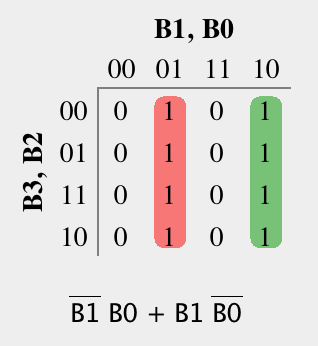
\includegraphics[width=0.5\textwidth]{media/SysLogiques/gray0.png}
    \centering
    \caption{Codage de Gray : $G_0$}
    \label{fig:gray0}
\end{figure}

\begin{figure}
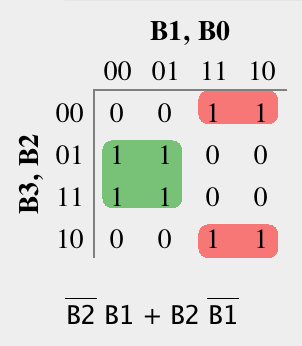
\includegraphics[width=0.5\textwidth]{media/SysLogiques/gray1.png}
    \centering
    \caption{Codage de Gray : $G_1$}
    \label{fig:gray1}
\end{figure}

\begin{figure}
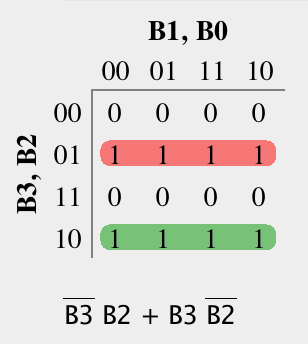
\includegraphics[width=0.5\textwidth]{media/SysLogiques/gray2.png}
    \centering
    \caption{Codage de Gray : $G_2$}
    \label{fig:gray2}
\end{figure}

\begin{figure}
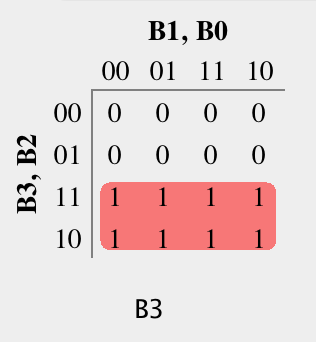
\includegraphics[width=0.5\textwidth]{media/SysLogiques/gray3.png}
    \centering
    \caption{Codage de Gray : $G_3$}
    \label{fig:gray3}
\end{figure}

À partir de ces expression optimisées, nous pouvons établir :
\[G_0 = \overline{B_1}\cdot B_0 + B_1 \cdot \overline{B_0} = B_0 \oplus B_1\]
\[G_1 = \overline{B_2}\cdot B_1 + B_2 \cdot \overline{B_1} = B_1 \oplus B_2\]
\[G_2 = \overline{B_3}\cdot B_2 + B_3 \cdot \overline{B_2} = B_2 \oplus B_3\]
\[G_3 = B3\]

\subsection{Codage Gray vers binaire}

Comme nous l'avons vu dans le chapitre sur la représentation binaire, paragraphe Codage de Gray, le codage inverse est très similaire puisqu'il suit l'équation :
\[B_n = G_0 \oplus G_1 \oplus G_2 \oplus ... \oplus G_n \]
Ce qui nous donne un enchaînement quasi évident de portes logiques XOR (ou exclusif).

\section{Bascules}
Jusque-là nous n'avons que des systèmes qui produisent une sortie pour une entrée donnée. Pour réaliser une \textit{machine} qui suive un \textbf{programme}, il nous faut un dispositif qui nous permette de stocker des résultats ou le programme lui-même.

\subsection{Verrou RS}
Un verrou RS possède deux entrées : \textbf{set} et \textbf{reset} ainsi que deux sorties dont l'une est l'inverse de l'autre : $Q$ et $\overline{Q}$. Le dispositf fonctionne de la manière suivante :
\begin{itemize}
    \item mise à 1 de $S$ (Set) : la sortie $Q$ passe à 1 ;
    \item mise à 1 de $R$ (Reset) : la sortie $Q$ passe à 0 ;
    \item $R$ = $S$ = 0 : état mémoire : la sortie $Q$ maintient sa valeur précédente $q$.
\end{itemize}
Pour représenter un tel système, nous allons proposer une table de vérité un peu particulière.
\\
\\
 \begin{tabular}{|c|c||c|c||c|}
    \hline
         \multicolumn{2}{|c||}{Entrées}& \multicolumn{2}{c||}{Sorties}&
         Remarques\\
        
         $S$ & $R$ & $Q$ & $\overline{Q}$ & \\
    \hline 
        0 & 0 & $q$ & $\overline{q}$ & mémoire \\
        0 & 1 & 0 & 1 & mise à 1 \\
        1 & 0 & 1 & 0 & mise à 0 \\
        1 & 1 & 0 & 0 & état interdit \\
    \hline
  \end{tabular}
\\

Un tel circuit est représenté sur la figure \ref{fig:basculeRS}

\begin{figure}
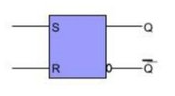
\includegraphics[width=0.5\textwidth]{media/SysLogiques/VerrouRS.png}
    \centering
    \caption{Verrou RS}
    \label{fig:basculeRS}
\end{figure}

Il peut être implémenté de deux manières différentes avec des portes NON-ET ou NON-OR comme on peut le voir sur les figures \ref{fig:vRS_NOR} et \ref{fig:vRS_NAND}

\begin{figure}
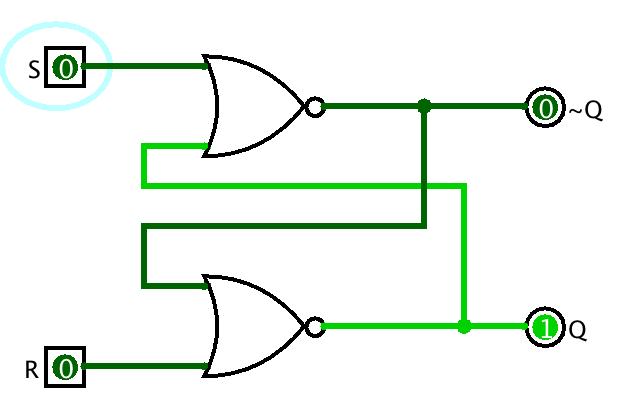
\includegraphics[width=0.5\textwidth]{media/SysLogiques/verrouRS_NOR.png}
    \centering
    \caption{Verrou RS avec des portes NOR}
    \label{fig:vRS_NOR}
\end{figure}

\begin{figure}
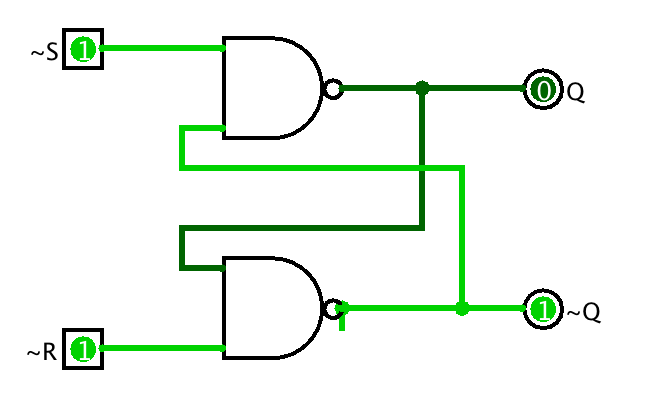
\includegraphics[width=0.5\textwidth]{media/SysLogiques/verrouRS_NAND.png}
    \centering
    \caption{Verrou RS avec des portes NAND}
    \label{fig:vRS_NAND}
\end{figure}


Il existe d'autres bascules plus élaborées que nous n'aborderons pas ici... (pour le moment).

Il faut cependant retenir que les bascules permettent de créer des registres. Avec huit bascules, on peut ainsi créer un registre de un octet qui nous permettra de stocker par exemple des résultats intermédiaires.

\end{document}